% ==========================================================================
%  CS4059 Fundamentals of Computer Vision -- Assignment 1
%  Industrial Defect Inspection & Surface-Crack Detection via Custom Linear
%  Filtering and Edge Processing.
%
%  Shahoud Shahid (23i-2515), Section DS-A -- FAST-NUCES, Fall 2026
%
%  Build:  latexmk -pdf main.tex        (see report/README.md)
%  This is the 4-page submission report.  A longer technical companion with
%  full derivations, code listings and every figure is in supplementary.tex.
% ==========================================================================
\documentclass[conference]{IEEEtran}
\IEEEoverridecommandlockouts

% ==========================================================================
%  Shared preamble for the Assignment 1 report (IEEE conference class).
%  Kept separate from main.tex so the supplementary document can reuse it.
% ==========================================================================
\usepackage[T1]{fontenc}
\usepackage[utf8]{inputenc}
\usepackage{lmodern}
\usepackage{microtype}

\usepackage{amsmath,amssymb,bm}
\usepackage{graphicx}
\graphicspath{{figures/}{../output_images/}}
\usepackage{subcaption}
\captionsetup{font=small,labelfont=bf}
\captionsetup[sub]{font=footnotesize}

\usepackage{booktabs}
\usepackage{array}
\usepackage{multirow}
\usepackage{siunitx}
\sisetup{
  detect-weight          = true,
  detect-family          = true,
  table-number-alignment = center,
  group-digits           = false,
}
% Numbers are written already-rounded in the source; siunitx only typesets them.

\usepackage{xcolor}
\definecolor{codebg}{gray}{0.96}
\definecolor{codekw}{RGB}{0,80,160}
\definecolor{codecomment}{RGB}{110,110,110}
\definecolor{codestr}{RGB}{160,40,40}

\usepackage{listings}
\lstdefinestyle{py}{
  language=Python,
  backgroundcolor=\color{codebg},
  basicstyle=\ttfamily\footnotesize,
  keywordstyle=\color{codekw}\bfseries,
  commentstyle=\color{codecomment}\itshape,
  stringstyle=\color{codestr},
  numbers=left, numberstyle=\tiny\color{codecomment}, numbersep=6pt,
  showstringspaces=false,
  breaklines=true,
  frame=single, framerule=0pt,
  columns=fullflexible,
  keepspaces=true,
  aboveskip=6pt, belowskip=4pt,
}
\lstset{style=py}

\usepackage[hidelinks]{hyperref}
\usepackage{xurl}  % allow URLs (e.g. in footnotes) to break at any character
\usepackage[nameinlink,capitalise]{cleveref}
\usepackage{enumitem}
\setlist{nosep,leftmargin=1.4em}

% Let TeX relax spacing rather than emit badness-10000 lines in the narrow
% two-column measure (unbreakable \code{} / \SI{} tokens are the usual cause).
\emergencystretch=3em
\hbadness=9000  % silence mild loose-line reports; genuine badness-10000 still shows

% Figure-heavy paper: allow denser float packing than the LaTeX defaults.
\setcounter{topnumber}{4}
\setcounter{bottomnumber}{2}
\setcounter{totalnumber}{5}
\renewcommand{\topfraction}{0.92}
\renewcommand{\bottomfraction}{0.7}
\renewcommand{\textfraction}{0.06}
\renewcommand{\floatpagefraction}{0.82}

% ----- project-wide macros ------------------------------------------------
\newcommand{\code}[1]{\texttt{\small #1}}
\newcommand{\conv}{\ensuremath{*}}
\newcommand{\R}{\ensuremath{\mathbb{R}}}
\newcommand{\Sx}{\ensuremath{S_x}}
\newcommand{\Sy}{\ensuremath{S_y}}
\newcommand{\Thi}{\ensuremath{T_{\text{high}}}}
\newcommand{\Tlo}{\ensuremath{T_{\text{low}}}}
\newcommand{\grad}{\ensuremath{\nabla}}
\newcommand{\Fout}{\ensuremath{F_{\text{sharp}}}}

% Consistent references to the two datasets
\newcommand{\PCB}{\textsc{pcb-defect}}
\newcommand{\CRACK}{\textsc{surface-crack}}


\begin{document}

\title{Industrial Defect Inspection and Surface-Crack Detection\\
via Custom Linear Filtering and First-Principles Canny Edge Processing}

\author{%
  \IEEEauthorblockN{Shahoud Shahid}
  \IEEEauthorblockA{Roll No.\ 23i-2515 \quad Section DS-A\\
    Department of Artificial Intelligence and Data Science\\
    FAST National University of Computer and Emerging Sciences\\
    \texttt{shahoudshahid652@gmail.com}}
}

\maketitle

\begin{abstract}
We implement an industrial visual-inspection pipeline from mathematical first
principles in vectorised NumPy: generalised 2-D/3-D convolution engines, an
isotropic Gaussian generator, unsharp masking, max/average pooling with
analytical gradients, and an exact four-stage Canny edge detector (Sobel
gradients, 4-sector non-maximum suppression, double thresholding, 8-connected
hysteresis). No built-in filtering primitive (\code{cv2.filter2D},
\code{cv2.Sobel}, \code{cv2.Canny}) is used. Benchmarking on \PCB{} and
\CRACK{} imagery, ablations quantify each stage: Gaussian pre-smoothing cuts the
gradient-noise standard deviation by up to $4.7\times$; non-maximum suppression
thins gradient bands by $8.1\times$; and double-threshold hysteresis lifts
crack-detection $F_1$ from $0.943$ to $0.988$ while reducing the number of
disconnected fragments from $40$ to $12$. We verify Witkin scale-space
causality, map the $(\Thi,\Tlo)$ operating regime on a $3\times3$ grid, and
analyse two Canny failure modes.
\end{abstract}

\begin{IEEEkeywords}
convolution, Canny edge detection, non-maximum suppression, hysteresis,
scale space, crack detection, defect inspection, NumPy.
\end{IEEEkeywords}

\section{Introduction}
\label{sec:intro}

Automated surface inspection is the first line of defence in high-precision
manufacturing (solar cells, silicon wafers, turbine blades) and in structural
health monitoring of concrete. Field imagery is degraded by shot noise, motion
blur and non-uniform illumination, so a robust inspection pipeline must combine
noise attenuation, contrast enhancement and sub-pixel-stable edge localisation.

This work builds that pipeline from scratch, following the classical
formulations of Canny~\cite{canny1986} and Gaussian scale
space~\cite{witkin1983,lindeberg1994}. Every operator is derived from its
defining equation in pure vectorised NumPy~\cite{harris2020numpy}; OpenCV is
restricted to image \emph{I/O}. The contributions are:
(i) strided \code{conv2d}/\code{conv3d} engines that satisfy the discrete
spatial-size formula exactly, as a single \code{einsum} over a sliding-window
view (\cref{sec:conv}); (ii) a closed-form unit-gain Gaussian, unsharp masking,
and max/average pooling with analytical back-propagation matrices
(\cref{sec:enh}); (iii) a four-stage Canny detector --- normalised Sobel,
vectorised 4-sector NMS, and 8-connected hysteresis (two implementations,
asserted equal) --- in \cref{sec:canny}; and (iv) stage-wise ablations with
tolerance-aware $P/R/F_1$ against ground truth, a $(\Thi,\Tlo)$ sensitivity
grid, a check of scale-space causality, and two failure-mode analyses
(\cref{sec:results,sec:failure}).

\section{Methods}
\label{sec:methods}

\subsection{Generalised convolution engines}
\label{sec:conv}

For an input of spatial size $I$, filter size $F$, symmetric zero-padding $P$
and stride $S$, the output size is
\begin{equation}
  O = \left\lfloor \frac{I - F + 2P}{S} \right\rfloor + 1 .
  \label{eq:convsize}
\end{equation}
\code{conv2d(image, kernel, stride, padding)} supports \code{'same'}
($P=(F-1)/2$, size-preserving only at $S=1$) and \code{'valid'} ($P=0$). We use
spatial \emph{cross-correlation} (no kernel flip): standard in modern
CV~\cite{szeliski2022}, permitted by the brief, and reversible via a
\code{flip\_kernel} flag. The engine takes a read-only sliding-window view
$\mathcal{W}\in\R^{O_h\times O_w\times F\times F}$
(\code{sliding\_window\_view}), strides it, and contracts against the kernel in
one call: \code{einsum("ijhw,hw->ij", W, K)}. A $512^2$ image with a $5\times5$
kernel takes \SI{\approx3}{\milli\second}. The output shape matches
\cref{eq:convsize} for all seven test geometries in
\code{results/task1\_shape\_verification.json} (e.g.\ a $32\times32$ input, $F=5$,
\code{valid} $\rightarrow 28\times28$).

\code{conv3d} takes a volume $\R^{H\times W\times C}$ and $K$ kernels
$\R^{F\times F\times C}$; each filter multiplies element-wise across all $C$
channels and sums the $F\!\cdot\!F\!\cdot\!C$ products. A single
\code{einsum("ijhwc,khwc->ijk", W, stack)} evaluates all $K$ filters at once,
producing activations $\R^{O_h\times O_w\times K}$.

\subsection{Gaussian smoothing, unsharp masking, pooling}
\label{sec:enh}

\paragraph{Isotropic Gaussian}
\code{generate\_gaussian\_kernel\_2d} evaluates
\begin{equation}
  G_\sigma(x,y)=\frac{1}{2\pi\sigma^2}\exp\!\left(-\frac{x^2+y^2}{2\sigma^2}\right)
  \label{eq:gauss}
\end{equation}
on a \code{meshgrid} centred at the middle tap, then rescales so
$\sum_{x,y}G_\sigma=1$ exactly, removing the truncation error of the finite
window. Separable $1$-D passes give an identical result in $O(k)$ rather than
$O(k^2)$.

\paragraph{Unsharp masking}
The high-pass detail signal $F - F\conv G_\sigma$ is re-injected with gain
$\alpha$:
\begin{equation}
  \Fout = F + \alpha\,\bigl(F - F \conv G_\sigma\bigr),
  \label{eq:unsharp}
\end{equation}
clipped to $[0,255]$. With $\sigma=1.5,\ \alpha=1.2$ the high-frequency energy
(mean absolute Laplacian response) rises by \SI{13.5}{\percent} on \PCB{} and
\SI{10.8}{\percent} on \CRACK{}, sharpening trace edges and micro-cracks
without halo artefacts (\code{pad\_mode='reflect'}).

\paragraph{Pooling and its gradient}
\code{pool2d} reduces non-overlapping / strided windows by \code{max} or
\code{average}. For the $2\times2$ block from the brief,
\begin{equation}
  X=\begin{bmatrix} 8 & 7\\ 12 & 9\end{bmatrix},\qquad
  \text{max-pool}(X)=12 ,
\end{equation}
the analytical Jacobian of the scalar output w.r.t.\ each input is
\begin{equation}
  \frac{\partial\,\text{Output}}{\partial\,\text{Input}}
  =\begin{bmatrix} 0 & 0\\ 1 & 0\end{bmatrix}.
  \label{eq:maxpoolgrad}
\end{equation}
\emph{Why gradients route only to the maximum:} with
$\text{out}=\max_k x_k=x_{k^\star}$, perturbing the winner gives
$\partial\,\text{out}/\partial x_{k^\star}=1$, while perturbing any other
element (still below $x_{k^\star}$) does not change the maximum, so its
derivative is $0$. Max-pooling is locally a hard, input-dependent
\emph{selector}; average pooling instead spreads the gradient uniformly at
$1/(p_h p_w)=0.25$. \Cref{eq:maxpoolgrad} matches a finite-difference check to
\num{1e-6}.

\subsection{Four-stage Canny edge detector}
\label{sec:canny}

\paragraph{Stage 1 -- gradients}
The grayscale image (BT.601 luma) is optionally Gaussian pre-smoothed, then
convolved with the normalised Sobel operators
\begin{equation}
  \Sx=\tfrac{1}{8}\!\begin{bmatrix}-1&0&1\\-2&0&2\\-1&0&1\end{bmatrix},\ \
  \Sy=\tfrac{1}{8}\!\begin{bmatrix}1&2&1\\0&0&0\\-1&-2&-1\end{bmatrix},
\end{equation}
giving magnitude $M=\sqrt{\Sx^2+\Sy^2}$ and orientation
$\theta=\operatorname{atan2}(\Sy,\Sx)$. Reflect padding avoids spurious border
gradients.

\paragraph{Stage 2 -- non-maximum suppression}
$\theta$ is mapped to $[0,180)^{\circ}$ and quantised into four sectors
($0,45,90,135^{\circ}\!\pm\!22.5^{\circ}$). A pixel is kept only if $M$ is
\emph{strictly greater} than both neighbours along the gradient direction
(horizontal, diagonal, vertical, anti-diagonal respectively); borders are
zeroed. The test is vectorised by pre-shifting eight padded copies of $M$ and
selecting per-sector with \code{np.select}, so NMS is $O(HW)$ with no Python
loop.

\paragraph{Stage 3 -- double threshold + hysteresis}
Pixels are \emph{strong} ($M\!\ge\!\Thi$), \emph{weak}
($\Tlo\!\le\!M\!<\!\Thi$) or non-edge; weak pixels are kept iff 8-connected
(directly or transitively) to a strong pixel. Two implementations are asserted
identical: a deque BFS flood-fill from the strong
seeds\ifdefined\SUPPLEMENTARY{} (\cref{lst:hyst})\fi, and a fixed-point
8-connected dilation constrained to \code{strong|weak}. Thresholds are absolute
or, by default, quantiles of the non-zero NMS response.

\ifdefined\SUPPLEMENTARY
\begin{lstlisting}[caption={8-connected hysteresis (BFS core).},label=lst:hyst,float=t]
q = deque(zip(*np.where(strong)))
out[strong] = 255
while q:
    ci, cj = q.popleft()
    for ni in range(max(0, ci-1), min(H, ci+2)):
        for nj in range(max(0, cj-1), min(W, cj+2)):
            if weak[ni, nj] and out[ni, nj] == 0:
                out[ni, nj] = 255
                q.append((ni, nj))
\end{lstlisting}
\fi

\section{Experimental Setup}
\label{sec:setup}

\paragraph{Datasets}
The brief specifies two Kaggle benchmarks: \PCB{}%
\footnote{\url{https://www.kaggle.com/datasets/akhatova/pcb-defects}}
(board defects: mouse bites, spurs, shorts, opens) and \CRACK{}%
\footnote{\url{https://www.kaggle.com/datasets/arunrk7/surface-crack-detection}}
(concrete cracks under diverse lighting). Both need credentials, so the loader
(\code{cvlab.datasets.get\_samples}) reads real images from \code{data/raw/}
when present and otherwise synthesises statistically-matched stand-ins:
orthogonal copper traces with pads and injected defects for \PCB{}; a
fractal-noise concrete surface with a radial illumination gradient and thin,
depth-modulated dark cracks for \CRACK{}. Each synthetic image ships an exact
ground-truth edge mask; \code{--data-dir} re-runs every experiment on the real
sets unchanged.

\paragraph{Metrics}
Against ground truth: tolerance-aware precision $P$, recall $R$, $F_1$ (a hit
within Chebyshev distance $2$). Reference-free: edge density, 8-connected
component count, mean component length.

\paragraph{Configuration}
Image size $256^2$, master seed \num{2515}, Gaussian pre-smoothing $\sigma=1.4$
unless stated; additive noise $\mathcal{N}(0,\sigma_n^2)$ in 8-bit units. The
full five-task suite runs in \SI{\approx16}{\second} on a laptop CPU.

\section{Results and Ablations}
\label{sec:results}

The assembled detector reaches $F_1=\num{0.931}$ on \PCB{}
($P=\num{1.000}$, $R=\num{0.871}$, 14 components) and $F_1=\num{1.000}$ on the
synthetic \CRACK{} sample. NMS collapses the gradient shoulder to a 1-px ridge
and hysteresis isolates the crack from background texture; the full per-stage
gallery (grayscale $\to$ smoothing $\to$ $|M|$ $\to$ orientation $\to$ NMS $\to$
strong/weak $\to$ hysteresis) for both benchmarks is in the supplementary.

\ifdefined\SUPPLEMENTARY
\begin{figure}[tb]
  \centering
  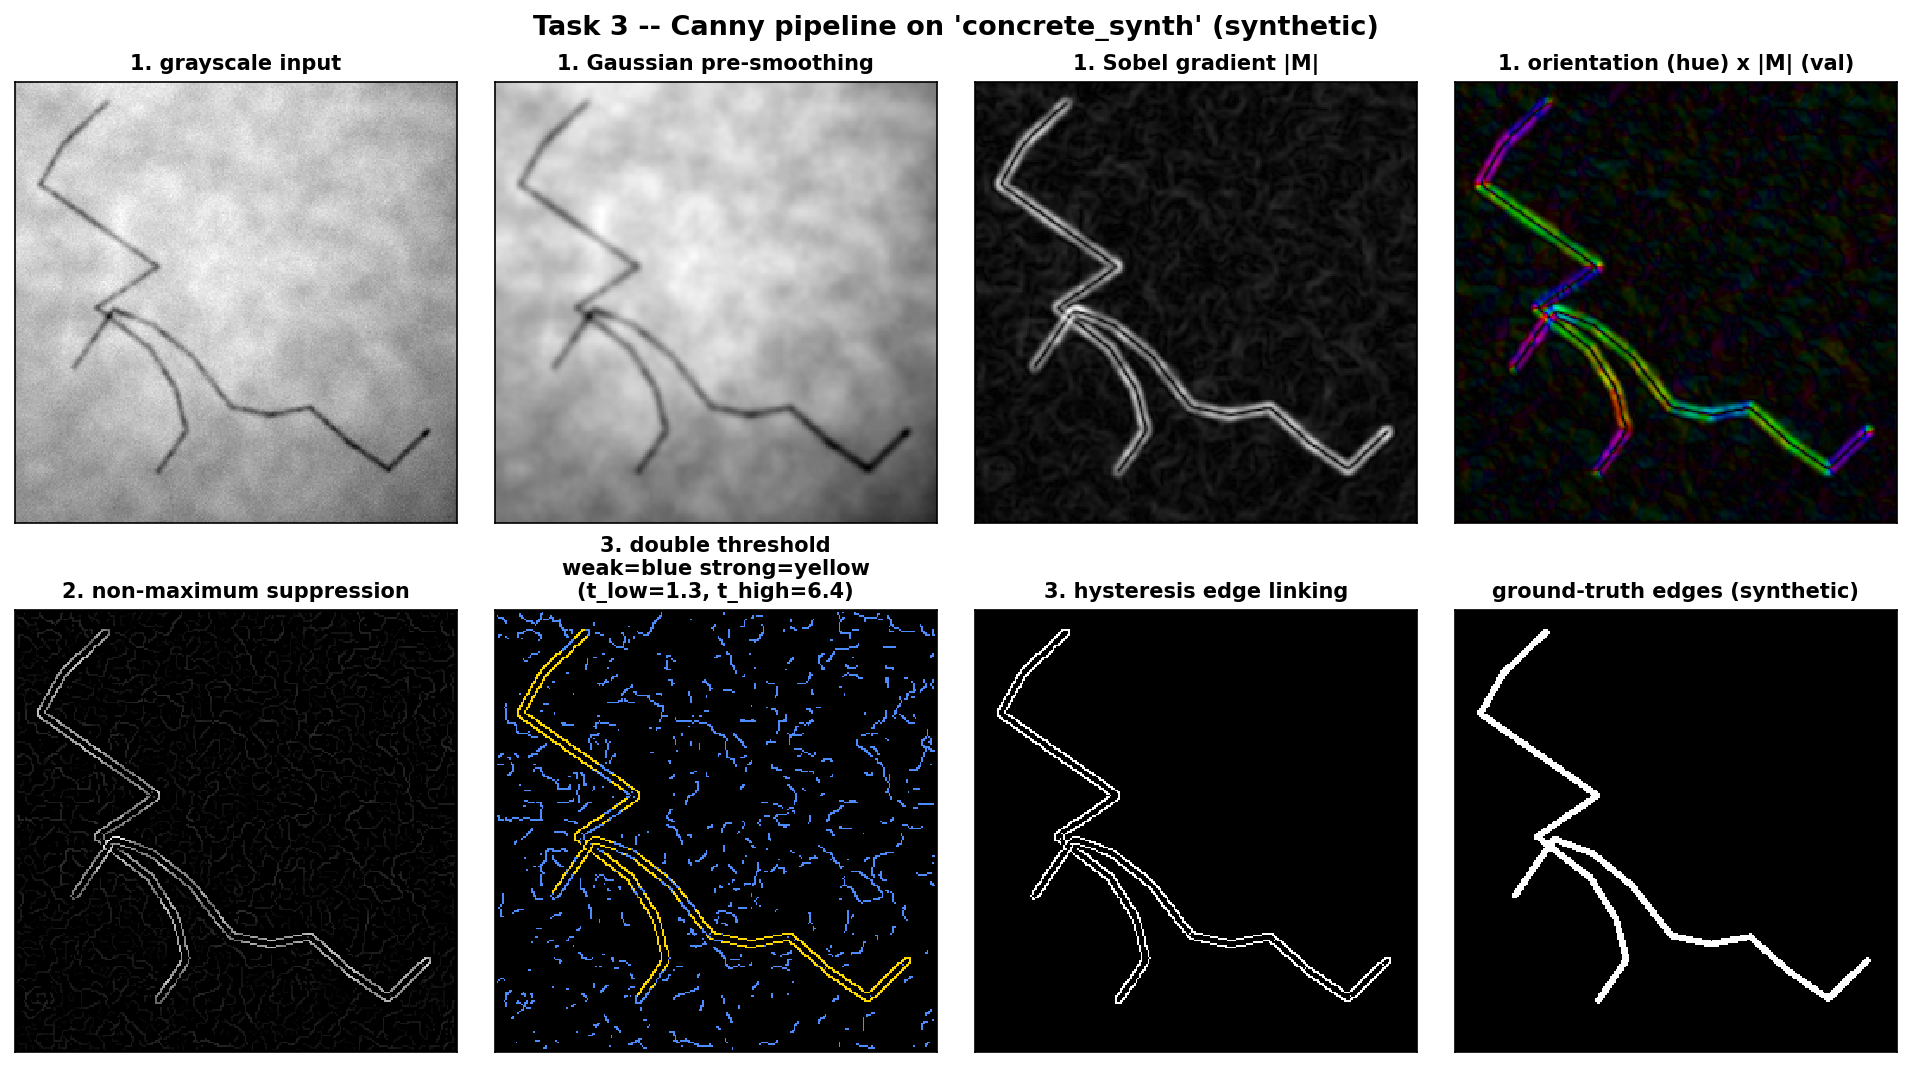
\includegraphics[width=\linewidth]{task3_canny_concrete.png}
  \caption{Four-stage Canny on a concrete-crack sample: grayscale, Gaussian
  pre-smoothing, Sobel $|M|$, orientation (hue)$\times|M|$ (value), NMS,
  double-threshold classes (weak = blue, strong = yellow), hysteresis, ground
  truth.}
  \label{fig:pipeline}
\end{figure}
\fi

\subsection{Ablation 1 -- noise and Gaussian pre-smoothing}
Differentiating a noisy image amplifies the noise: the gradient-magnitude std.\
dev.\ grows with $\sigma_n$ as $3.50\!\to\!7.30\!\to\!11.42$ for
$\sigma_n\in\{10,25,40\}$. A single Gaussian pass ($\sigma=1.4$) holds it at
$1.47\!\to\!1.79\!\to\!2.42$ --- a noise-suppression ratio rising from
\SI{2.4}{\times} to \SI{4.7}{\times} --- while keeping the crack ridge intact
(\cref{fig:abl1}). This is the derivative-of-noise argument for Stage 1.

\begin{figure}[tb]
  \centering
  \ifdefined\SUPPLEMENTARY
    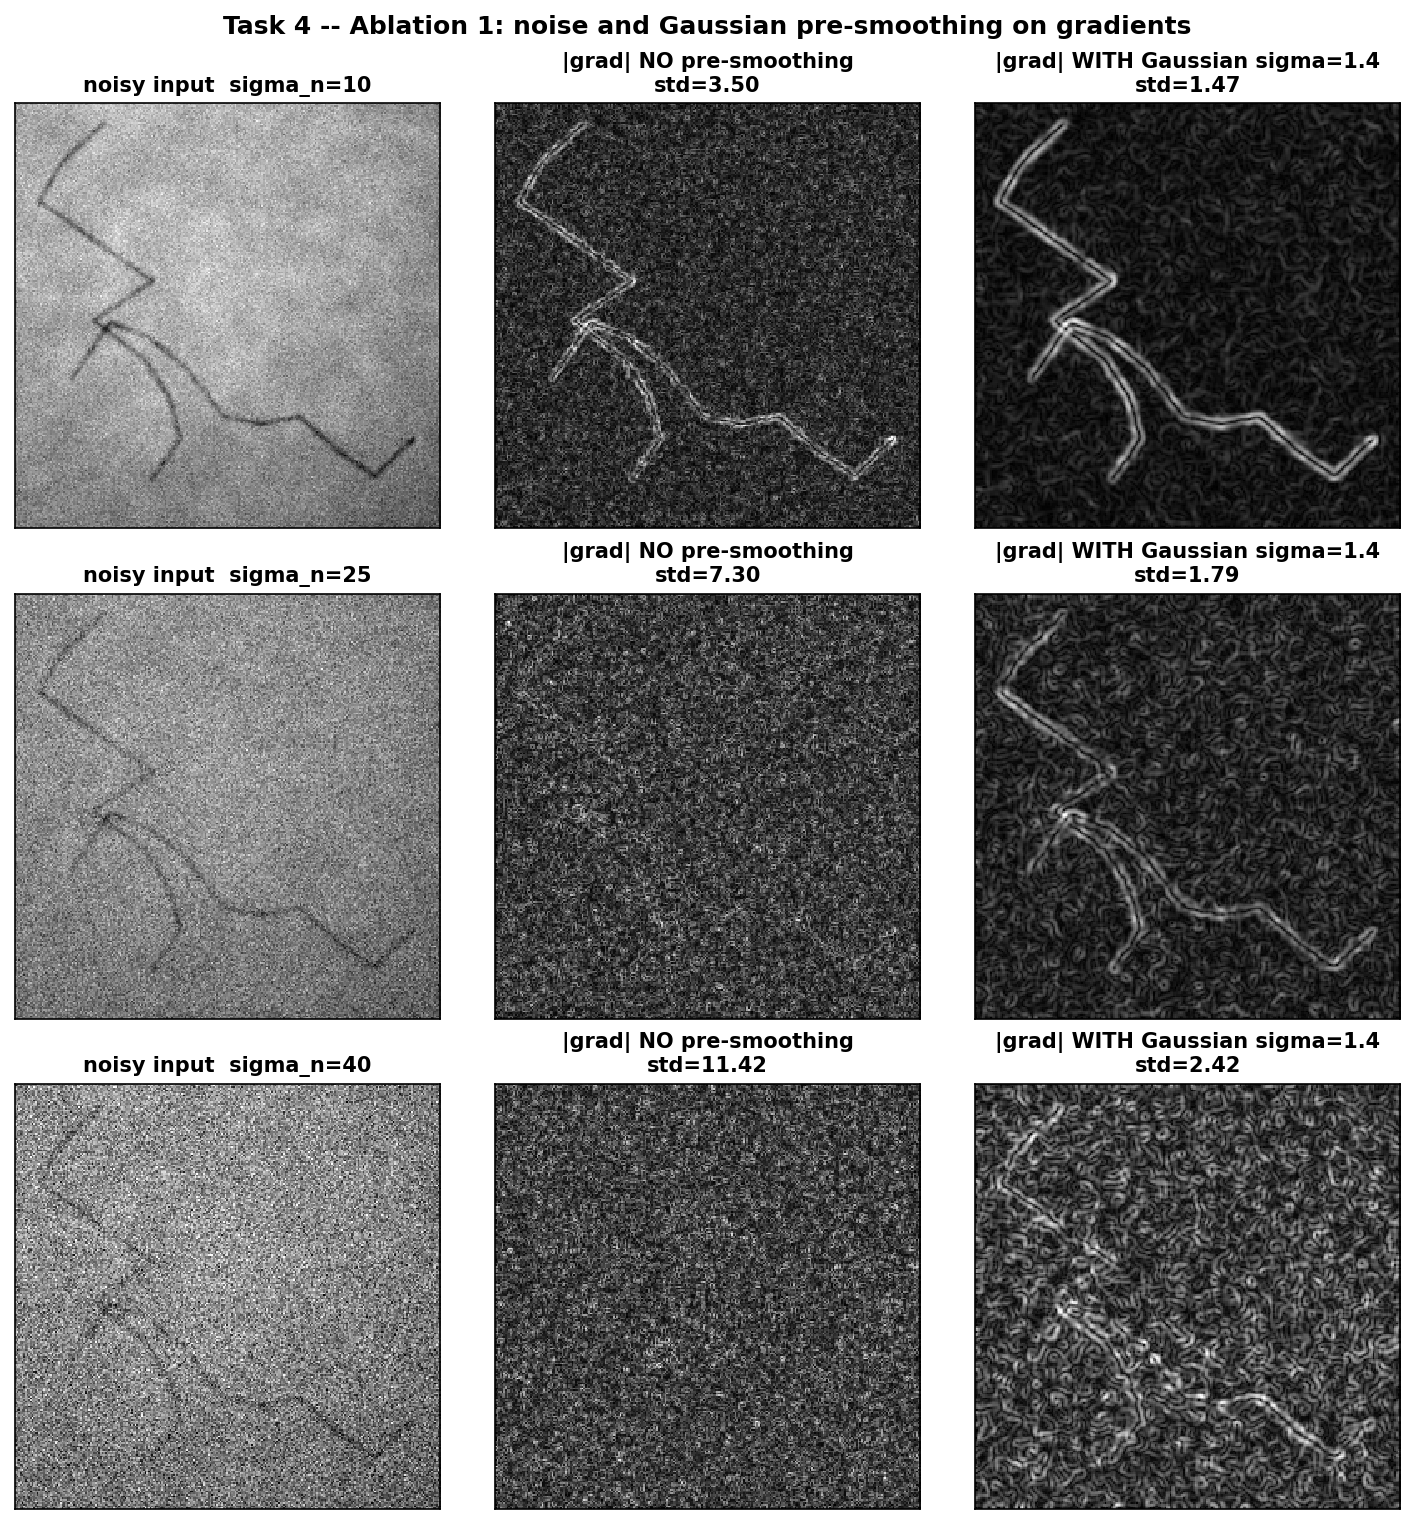
\includegraphics[width=0.86\linewidth]{task4_ablation1_noise_smoothing_full.png}
    \caption{Ablation 1. Rows: $\sigma_n\in\{10,25,40\}$. Columns: noisy input;
    $|\nabla|$ without pre-smoothing; $|\nabla|$ with Gaussian pre-smoothing.}
  \else
    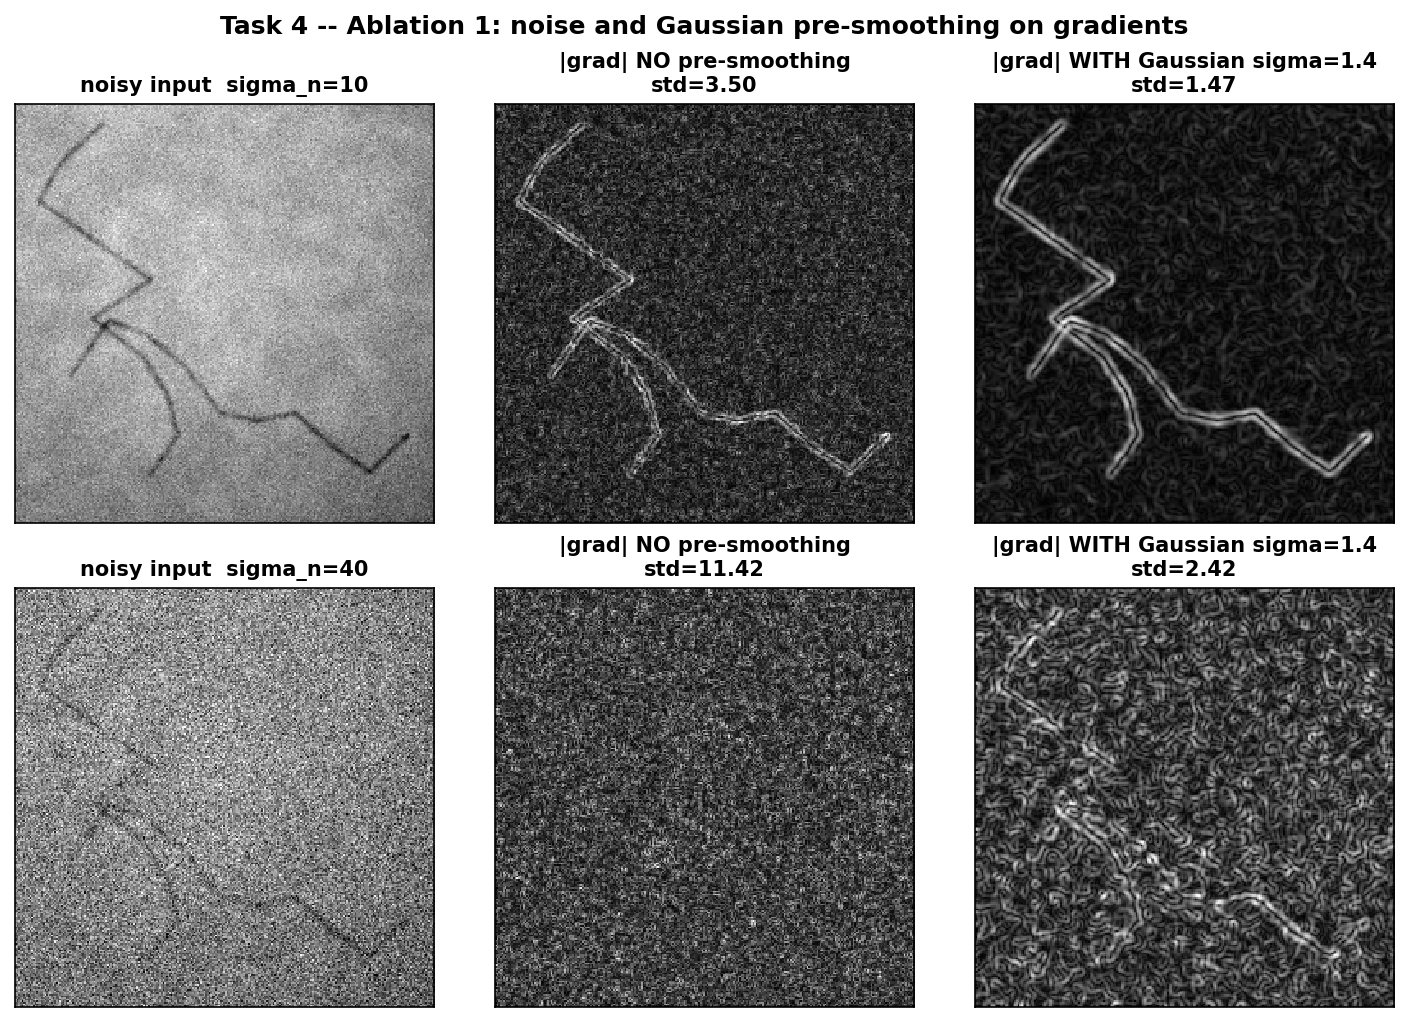
\includegraphics[width=0.82\linewidth]{task4_ablation1_noise_smoothing.png}
    \caption{Ablation 1 (extremes $\sigma_n\in\{10,40\}$; $\sigma_n{=}25$ in the
    supplementary). Columns: noisy input; $|\nabla|$ without pre-smoothing;
    $|\nabla|$ with Gaussian pre-smoothing.}
  \fi
  \label{fig:abl1}
\end{figure}

\subsection{Ablation 2 -- non-maximum suppression}
Thresholding the (over-smoothed) gradient magnitude directly yields thick bands
covering \SI{40.0}{\percent} of the frame; applying the same threshold
\emph{after} NMS yields 1-px ridges at \SI{4.9}{\percent} density --- a
\SI{8.1}{\times} thinning (\cref{fig:abl2}).

\begin{figure}[tb]
  \centering
  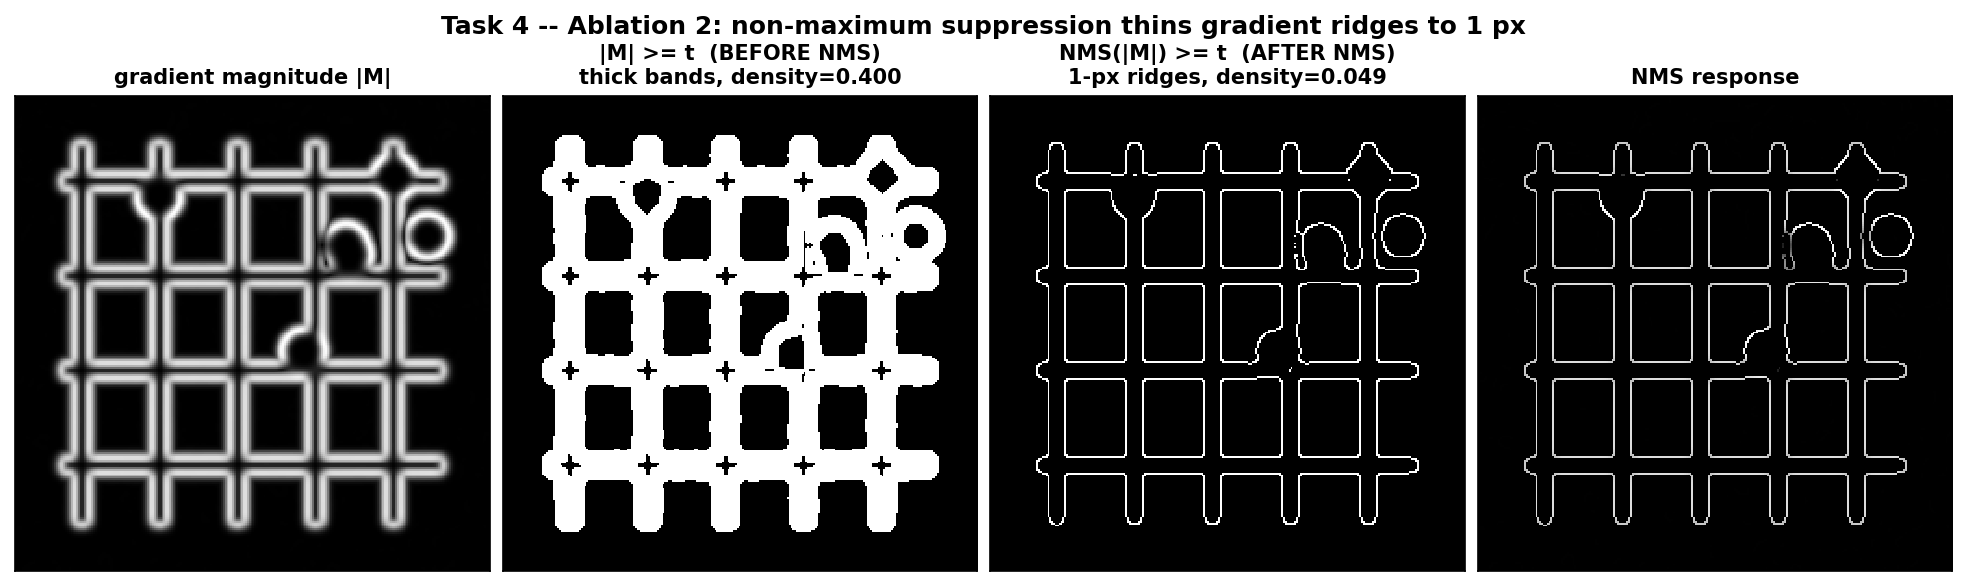
\includegraphics[width=0.9\linewidth]{task4_ablation2_nms.png}
  \caption{Ablation 2. $|M|\!\ge\!t$ before NMS (thick bands) vs.\
  $\mathrm{NMS}(|M|)\!\ge\!t$ (1-px ridges), same threshold $t$.}
  \label{fig:abl2}
\end{figure}

\subsection{Ablation 3 -- hysteresis vs.\ single threshold}
On a faint, contrast-varying crack in noise (\cref{fig:abl3},
\cref{tab:ablation3}): a single low threshold floods the background
($P=\num{0.535}$, 225 fragments); a single high threshold is clean but breaks
the crack ($R=\num{0.898}$, 40 fragments); double-threshold hysteresis links
the weak crack stretches to strong seeds while rejecting isolated texture,
reaching $F_1=\num{0.988}$ in only \textbf{12} connected components.

\begin{table}[t]
  \centering
  \caption{Ablation 3: single threshold vs.\ hysteresis (faint crack, $\sigma_n{=}12$).}
  \label{tab:ablation3}
  \small
  \setlength{\tabcolsep}{4pt}
  \begin{tabular}{lccccc}
    \toprule
    method & $P$ & $R$ & $F_1$ & density & \#comp. \\
    \midrule
    single @ $\Tlo$  & 0.535 & 1.000 & 0.697 & 0.019 & 225 \\
    single @ $\Thi$  & 0.993 & 0.898 & 0.943 & 0.006 & 40 \\
    \textbf{hysteresis} & 0.982 & 0.994 & \textbf{0.988} & 0.010 & \textbf{12} \\
    \bottomrule
  \end{tabular}
\end{table}

\begin{figure}[tb]
  \centering
  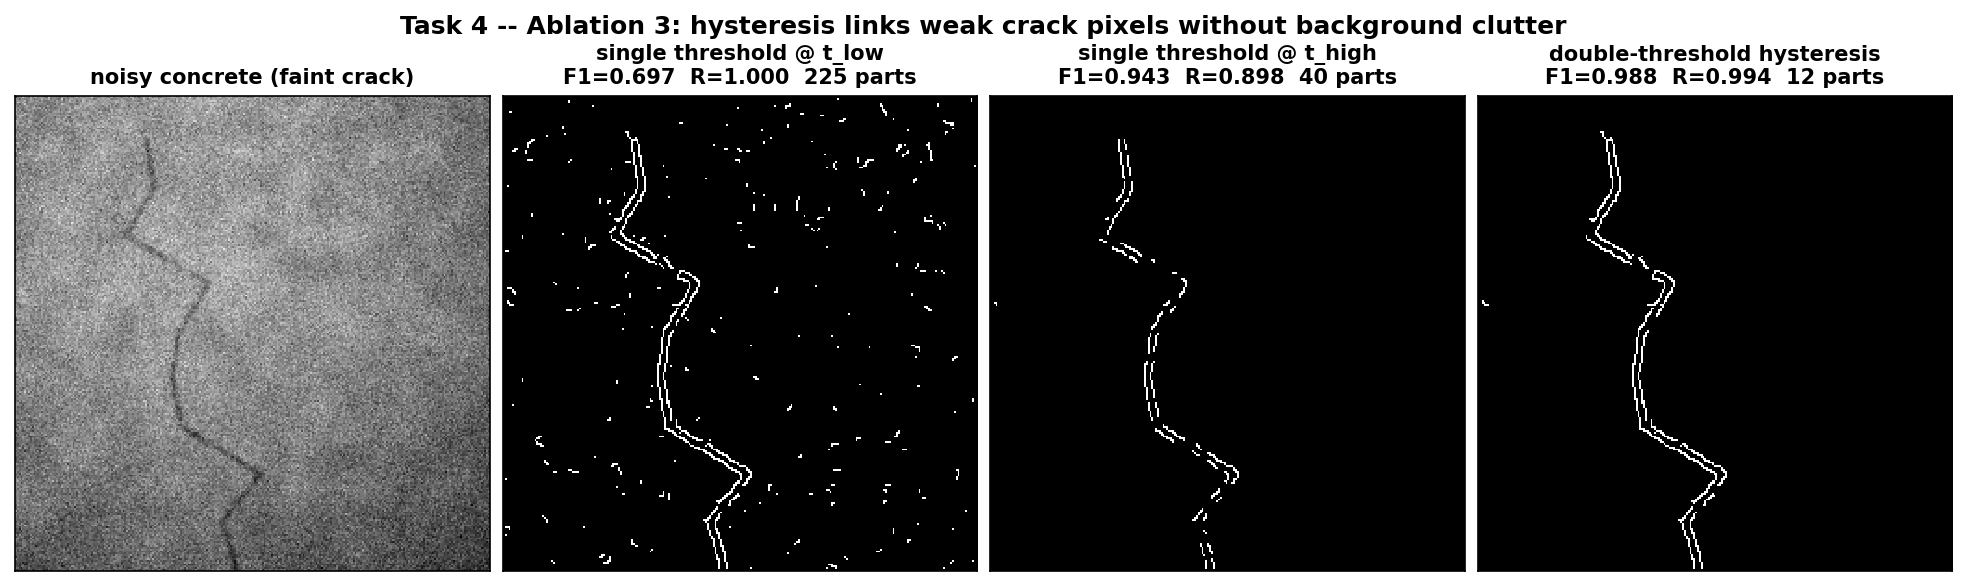
\includegraphics[width=0.92\linewidth]{task4_ablation3_hysteresis.png}
  \caption{Ablation 3. Left to right: noisy input; single threshold at $\Tlo$;
  single threshold at $\Thi$; double-threshold hysteresis.}
  \label{fig:abl3}
\end{figure}

\subsection{Scale-space causality}
\label{sec:scalespace}
Running the detector at $\sigma\in\{1.0,2.5,5.0\}$ gives edge counts
$2055 \to 1418 \to 881$ --- strictly decreasing (\cref{fig:scale}). Tracking
the second-derivative zero-crossings along a fixed scan-line over
$\sigma\in[0.4,8.0]$ likewise shows the count fall monotonically from
\num{120} to \num{15}.

\emph{Why edges only merge, never appear (Witkin
causality~\cite{witkin1983}).} Gaussian smoothing of a 1-D
signal is the heat equation $\partial_t u = \tfrac12\partial_{xx}u$ run for
time $t=\sigma^2$. Diffusion obeys a maximum principle: it cannot increase the
number of local extrema of $u$ or of any derivative $\partial_x^n u$. Edges are
zero-crossings of $\partial_{xx}(G_\sigma\conv f)$, so no new edge can be
created; existing zero-crossings drift and annihilate in pairs as neighbouring
extrema of $\partial_{xx}u$ merge. Every coarse-scale edge therefore has a
unique fine-scale ancestor, which is what makes coarse-to-fine tracking well
posed. (Full argument: supplementary, Appendix~A.)

\begin{figure}[tb]
  \centering
  \ifdefined\SUPPLEMENTARY
    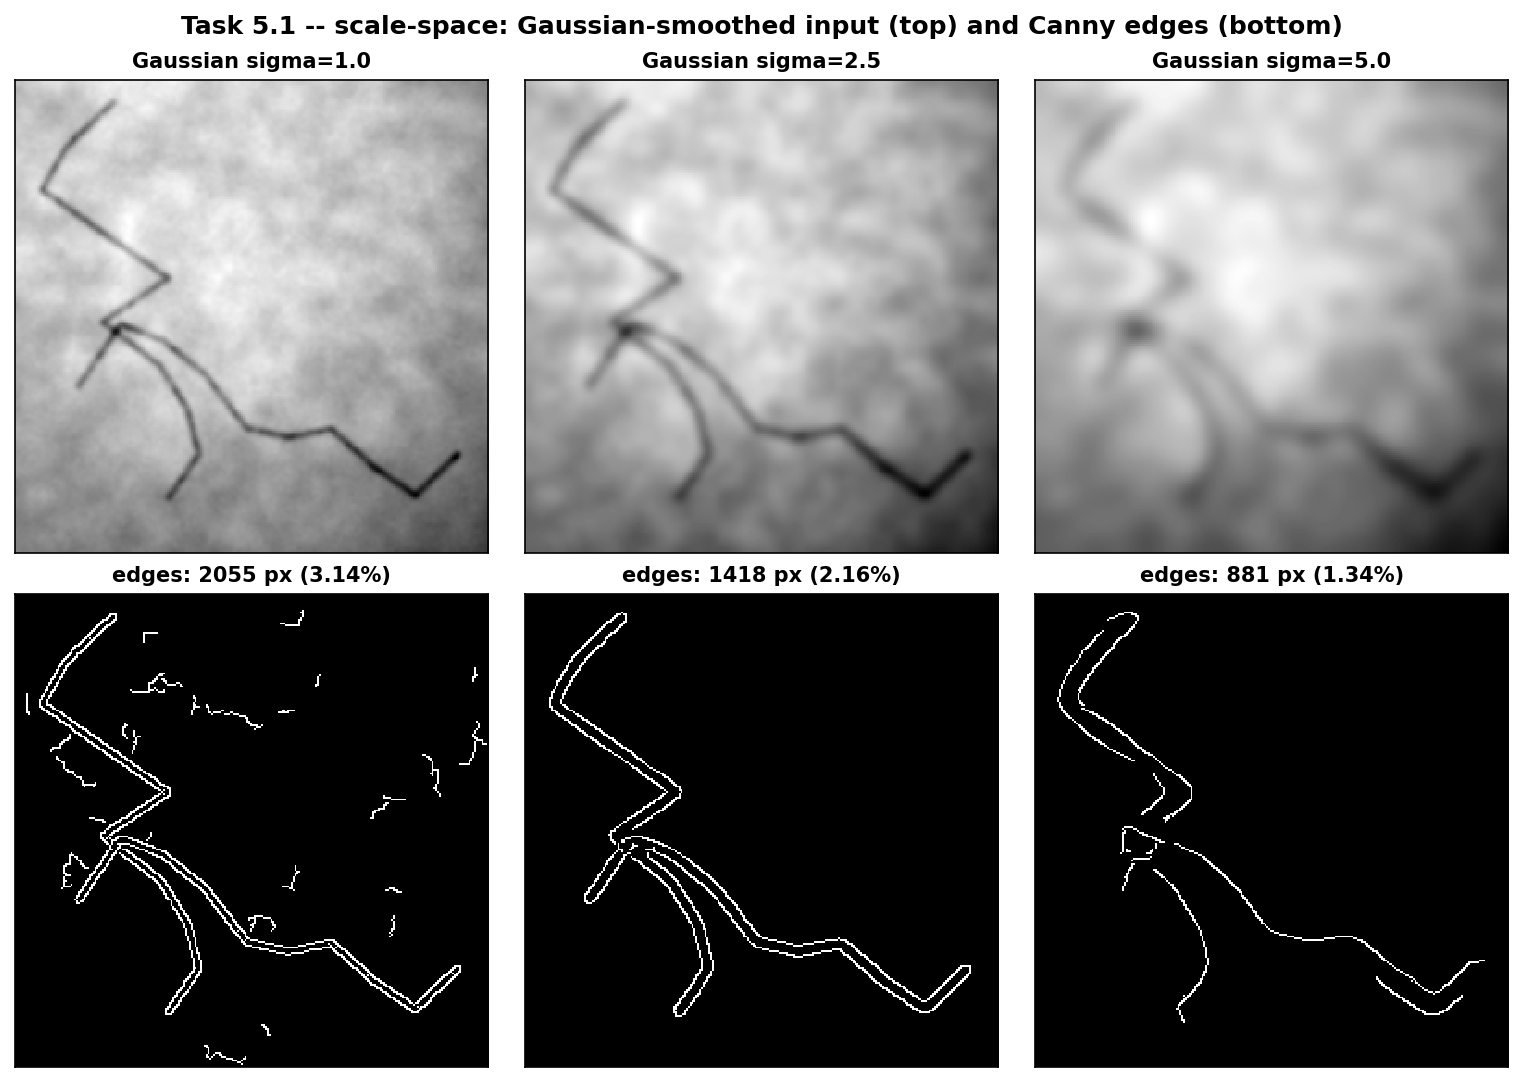
\includegraphics[width=\linewidth]{task5_scale_space_full.png}
  \else
    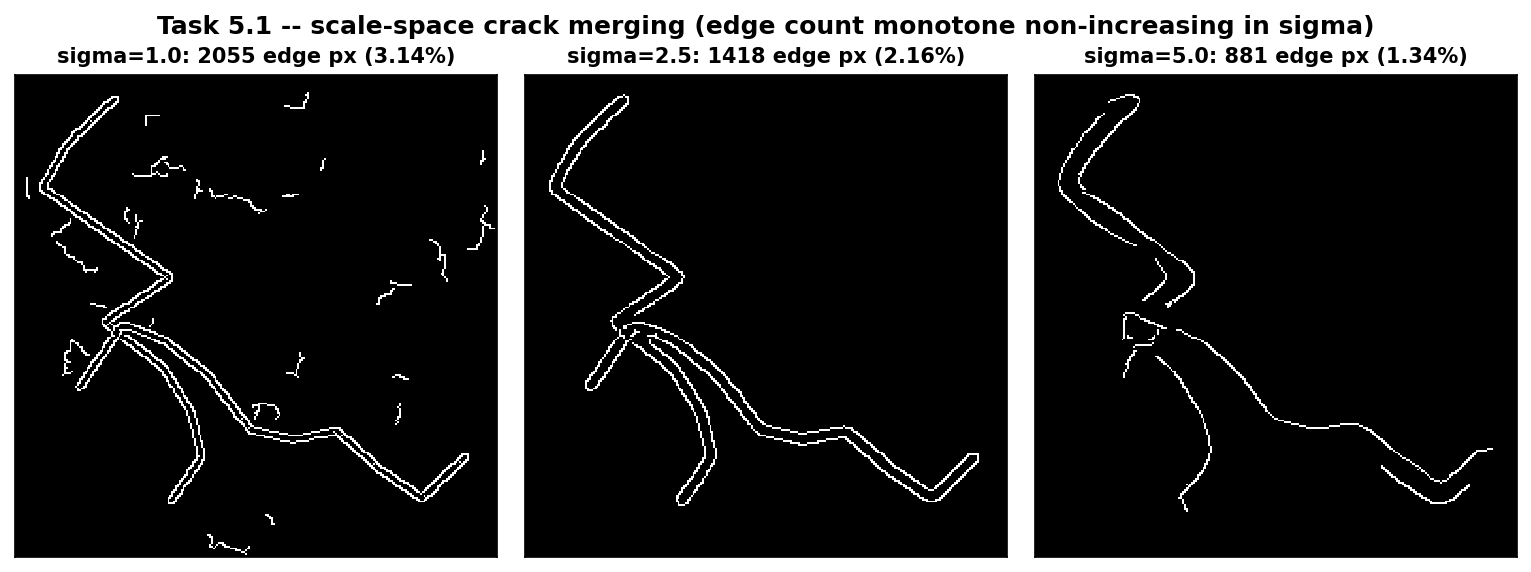
\includegraphics[width=\linewidth]{task5_scale_space.png}
  \fi
  \caption{Scale-space: increasing $\sigma$ destroys texture edges; the crack
  edges shift and merge but no new edges appear. Edge counts
  $2055 \to 1418 \to 881$.}
  \label{fig:scale}
\end{figure}

\ifdefined\SUPPLEMENTARY
\begin{figure}[tb]
  \centering
  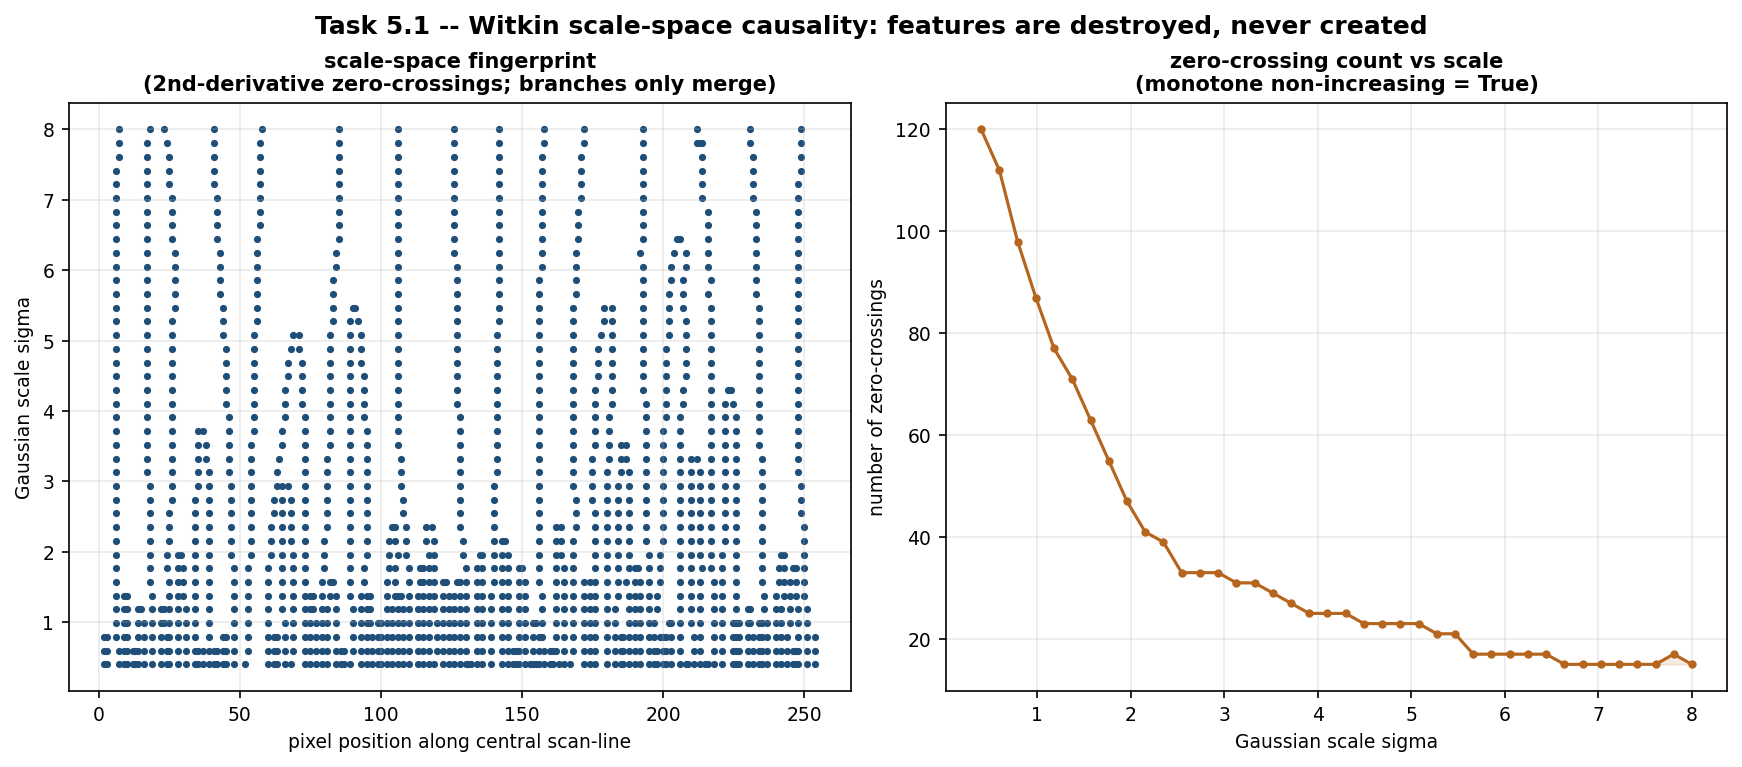
\includegraphics[width=\linewidth]{task5_scale_space_causality.png}
  \caption{Left: zero-crossing fingerprint (branches only merge upward).
  Right: zero-crossing count is monotone non-increasing in $\sigma$.}
  \label{fig:causality}
\end{figure}
\fi

\subsection{Parameter sensitivity}
\label{sec:sensitivity}
We sweep $\Thi$ (quantiles $0.75/0.88/0.96$ of the NMS response) against
$\Tlo=\{0.3,0.5,0.8\}\,\Thi$ on noisy \CRACK{} and \PCB{} (full $3\times3$
edge-map grids in \cref{fig:grid}). \Cref{tab:grid} extracts the diagonal: a low
$\Thi$ admits texture regardless of $\Tlo$ ($F_1\!\approx\!0.15$); the usable
regime is a high $\Thi$ (top few percent of gradient energy) with $\Tlo$ at
\SIrange{50}{80}{\percent} of it ($F_1=\num{0.888}$), matching the classic
$2$--$3\!:\!1$ ratio heuristic. The \PCB{} grid peaks at $F_1=\num{0.936}$
($\Thi=\text{q}0.88$, $\Tlo=0.3\,\Thi$), reflecting its higher edge contrast.

\begin{table}[t]
  \centering
  \caption{Sensitivity diagonal, noisy \CRACK{} ($\sigma_n{=}25$); best in bold.
  Full $3\times3$ grids: \cref{fig:grid}.}
  \label{tab:grid}
  \small
  \setlength{\tabcolsep}{4.5pt}
  \begin{tabular}{llccc}
    \toprule
    $\Thi$ (quantile) & $\Tlo/\Thi$ & density & \#comp. & $F_1$ \\
    \midrule
    q0.75 & 0.30 & 0.291 & 227 & 0.151 \\
    q0.88 & 0.50 & 0.148 & 270 & 0.268 \\
    q0.96 & 0.30 & 0.082 & 39  & 0.436 \\
    q0.96 & 0.50 & 0.035 & 47  & 0.769 \\
    q0.96 & 0.80 & 0.020 & 77  & \textbf{0.888} \\
    \bottomrule
  \end{tabular}
\end{table}

\ifdefined\SUPPLEMENTARY
\begin{figure}[tb]
  \centering
  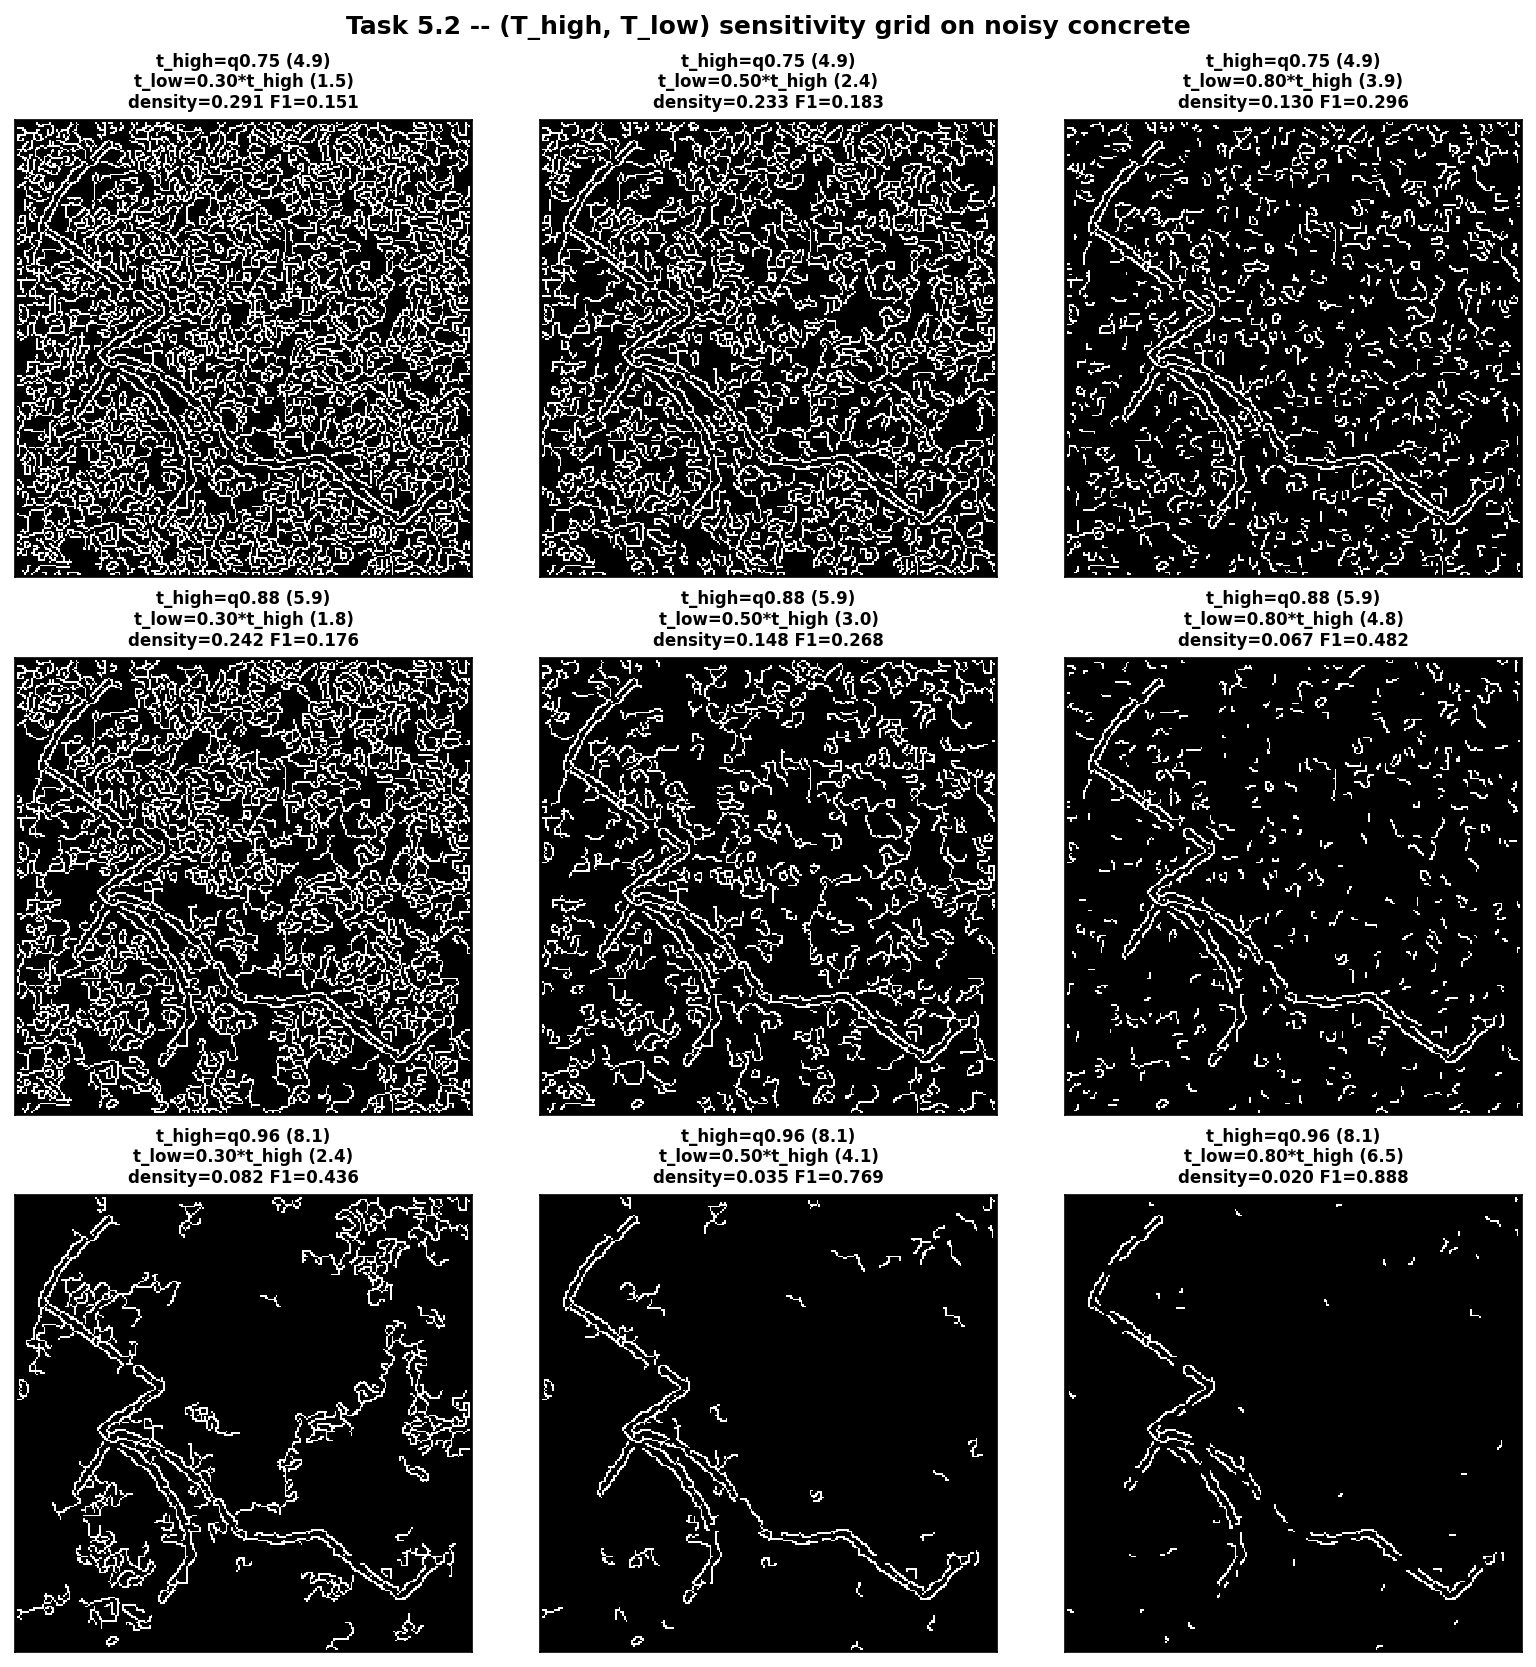
\includegraphics[width=\linewidth]{task5_sensitivity_grid_concrete.png}
  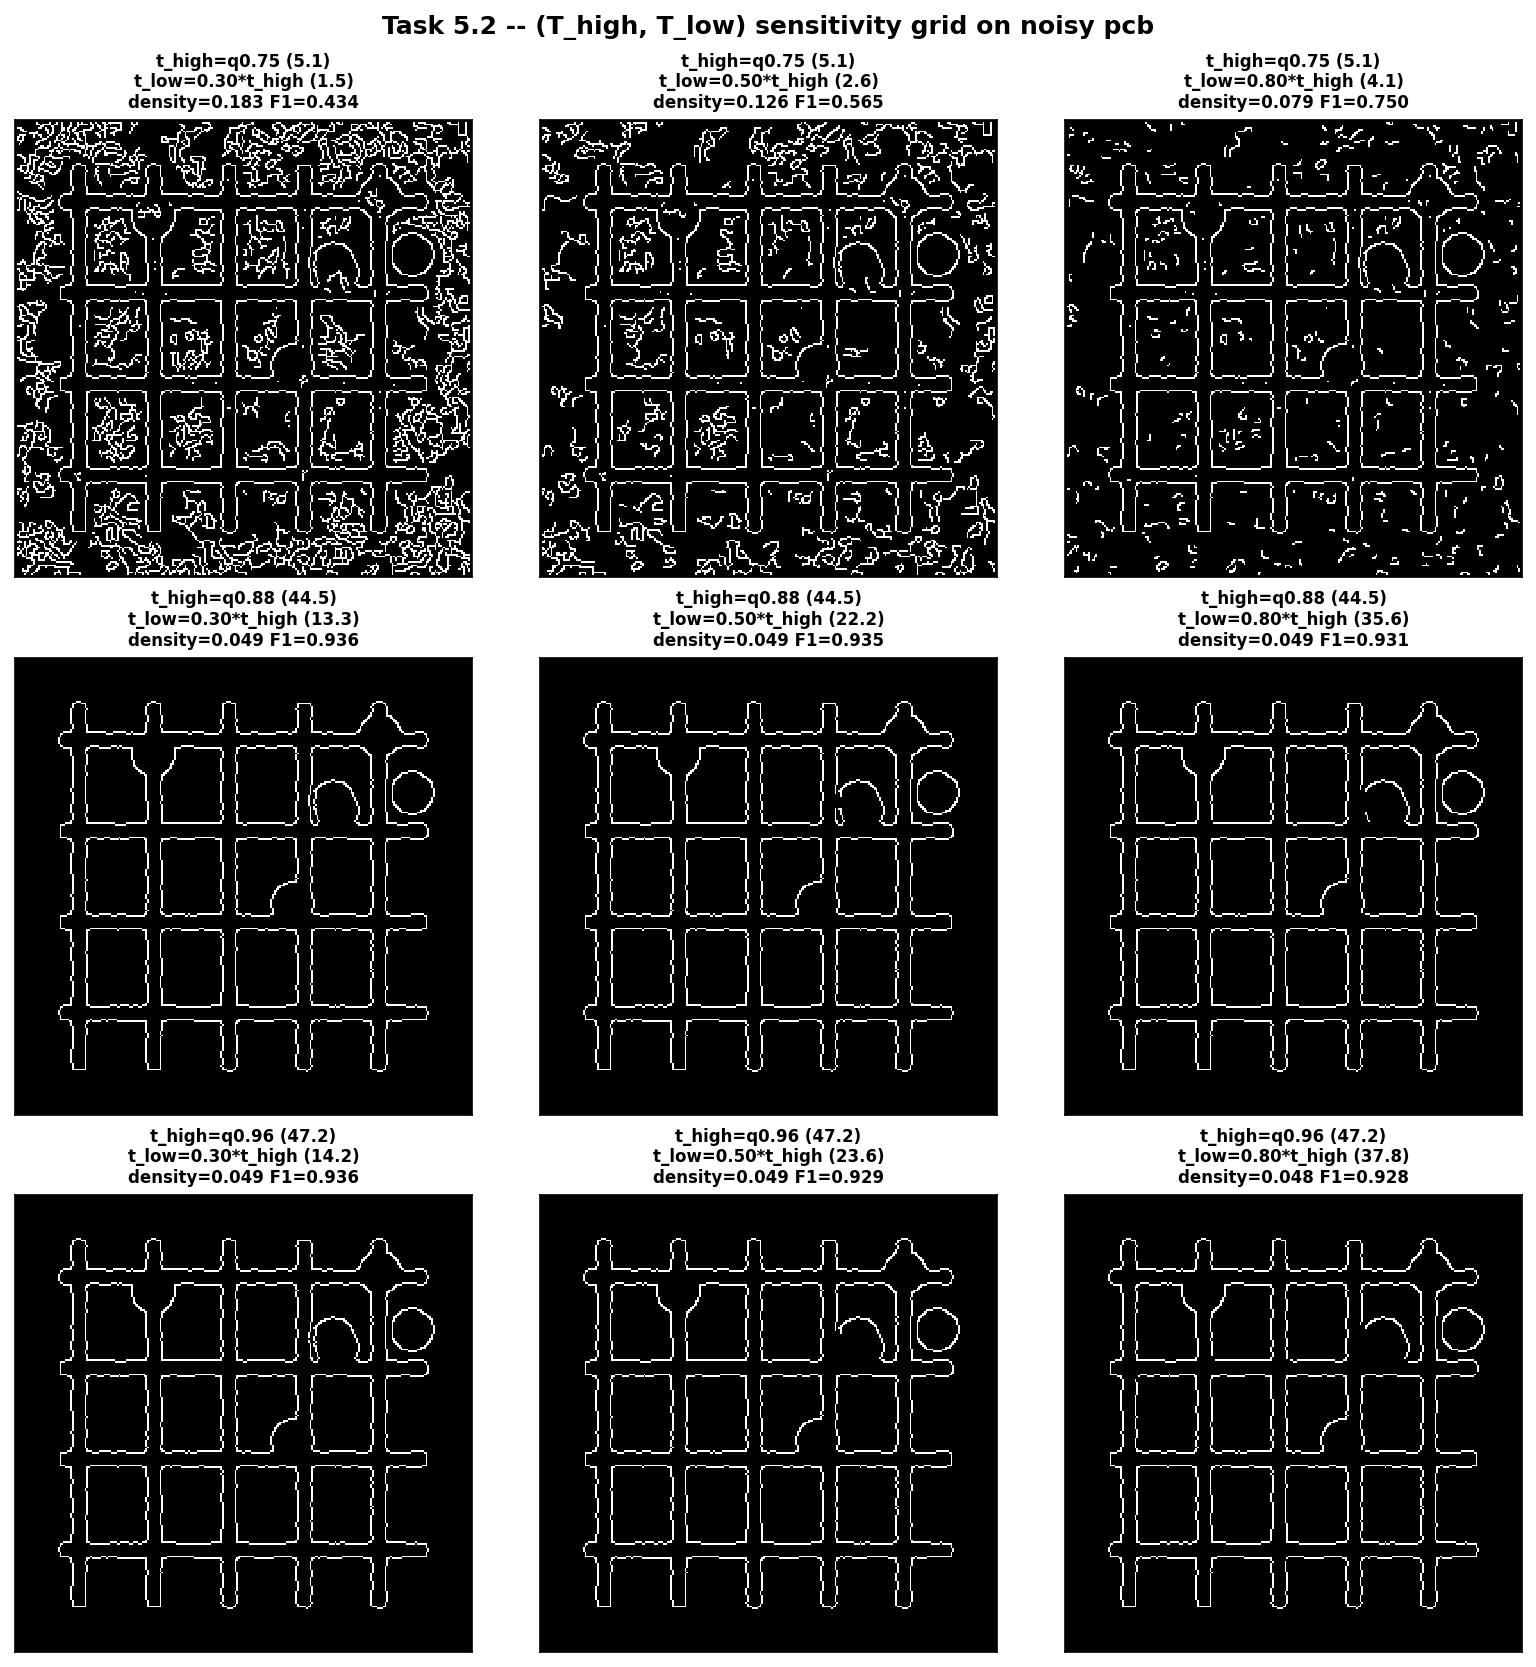
\includegraphics[width=\linewidth]{task5_sensitivity_grid_pcb.png}
  \caption{$3\times3$ $(\Thi,\Tlo)$ grids on noisy concrete (top) and PCB
  (bottom). Rows: $\Thi$ quantile increasing downward. Columns: $\Tlo/\Thi$
  increasing rightward.}
  \label{fig:grid}
\end{figure}
\else
\begin{figure}[tb]
  \centering
  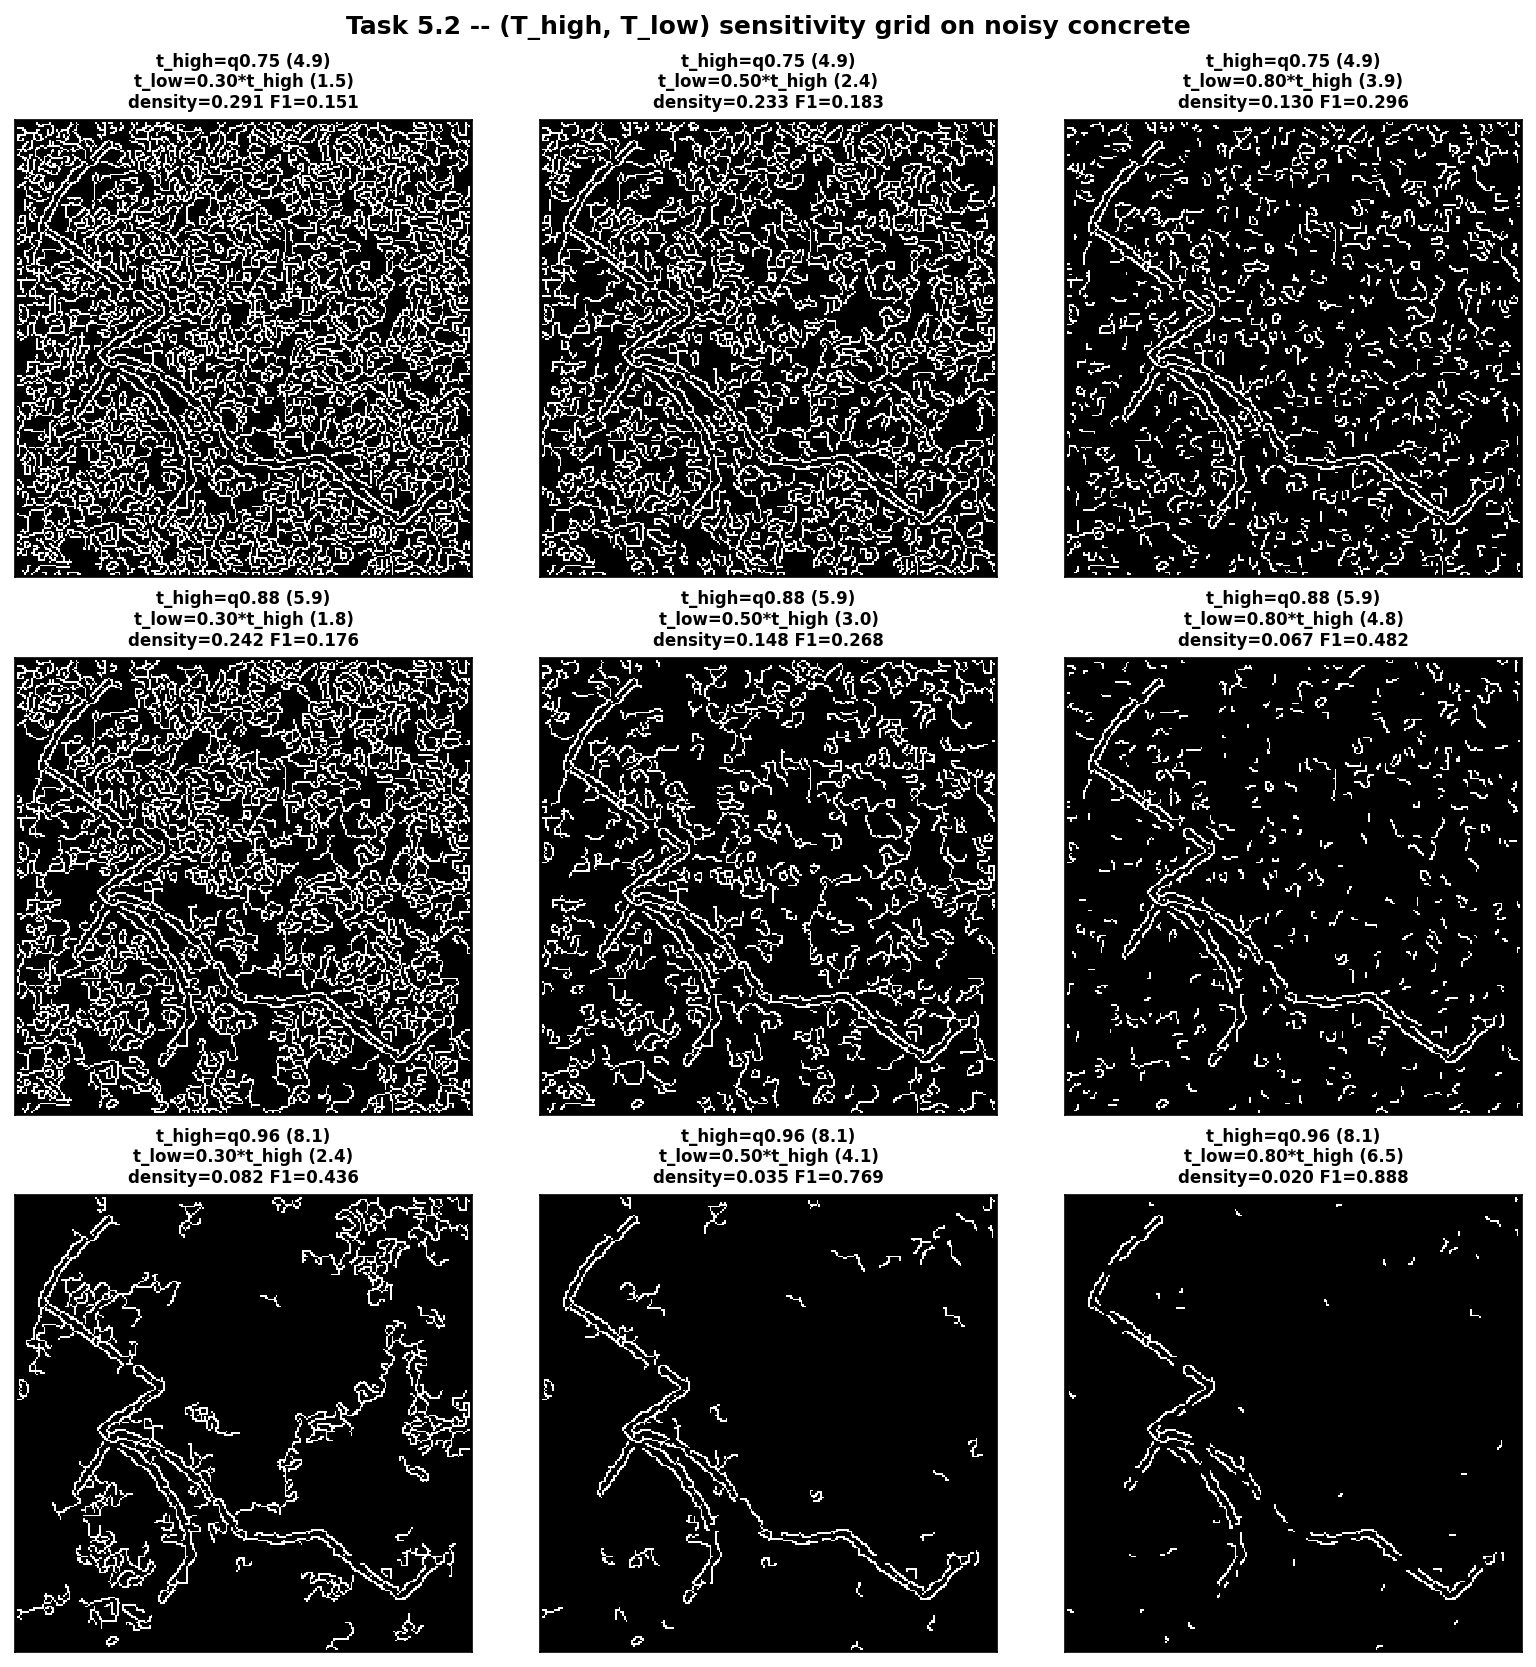
\includegraphics[width=0.9\linewidth]{task5_sensitivity_grid_concrete.png}
  \caption{$3\times3$ $(\Thi,\Tlo)$ grid on noisy concrete. Rows: $\Thi$
  quantile $\uparrow$ downward; columns: $\Tlo/\Thi$ $\uparrow$ rightward.
  PCB grid in the supplementary.}
  \label{fig:grid}
\end{figure}
\fi

\section{Failure Case Analysis}
\label{sec:failure}

\Cref{fig:fail} shows two scenarios where Canny --- a pure first-order-gradient
detector with no notion of semantics --- fails. In both, crack recall stays at
\num{1.0} but precision collapses ($P=\num{0.41}$ and $P=\num{0.35}$).

\paragraph{Strong cast-shadow contour}
A hard shadow boundary is a genuine intensity step, so it produces a Sobel
response \emph{larger} than the crack; NMS keeps it and no $(\Thi,\Tlo)$ removes
it without also removing the crack. The limitation is definitional: Canny
detects \emph{intensity} edges, but a shadow is an \emph{illumination} edge, not
surface geometry. Separating them needs illumination modelling (retinex /
homomorphic) or colour, which a single-channel gradient lacks.

\paragraph{High-frequency texture}
On coarse aggregate the surface is itself full of small intensity steps whose
magnitudes match the faint crack, so (i) no global threshold separates signal
from texture, and (ii) hysteresis worsens it --- the texture edges form a
percolating 8-connected web, so one strong seed floods large areas. The output
is an "edge soup" (73 components) in which the crack is not distinguishable by
connectivity. The limitation is scale: a fixed-$\sigma$ gradient cannot tell
which edges belong to a structure of interest. Remedies: oriented crack-matched
filters, multi-scale ridge measures (Frangi), or a learned segmenter.

\begin{figure}[tb]
  \centering
  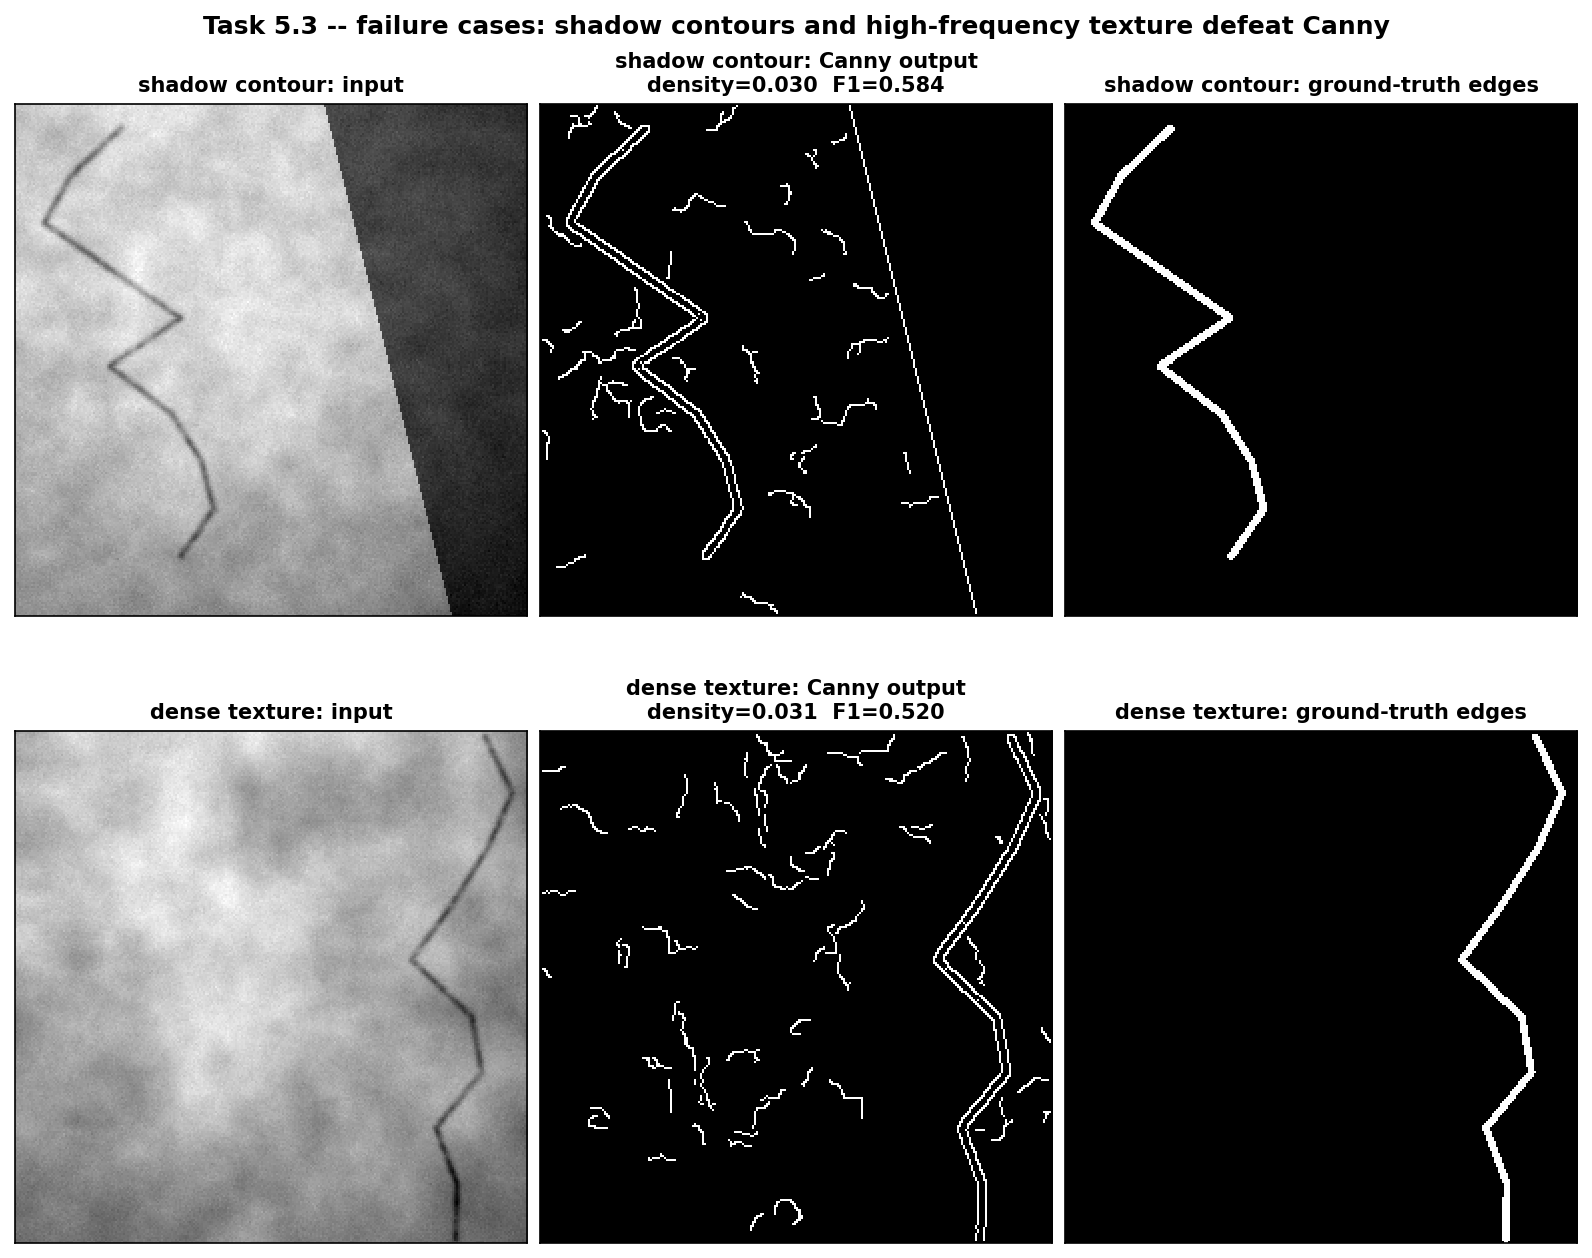
\includegraphics[width=0.7\linewidth]{task5_failure_cases.png}
  \caption{Failure cases. Row 1: a cast-shadow contour becomes a strong false
  edge. Row 2: dense texture yields a fragmented map that buries the crack.
  Columns: input, Canny output, ground truth.}
  \label{fig:fail}
\end{figure}

\section{Conclusion}
\label{sec:conclusion}

A complete inspection pipeline --- strided 2-D/3-D convolution, Gaussian and
unsharp filtering, pooling with analytical gradients, and an exact four-stage
Canny detector --- was built from first principles in vectorised NumPy and
validated by \num{124} unit tests. The ablations quantify each stage: Gaussian
pre-smoothing suppresses gradient noise up to \SI{4.7}{\times}; NMS thins ridges
\SI{8.1}{\times}; hysteresis raises crack $F_1$ to \num{0.988} with a
\SI{70}{\percent} drop in fragment count. Scale-space behaviour matches Witkin
causality and the $(\Thi,\Tlo)$ sweep confirms the high-$\Thi$,
$2$--$3\!:\!1$-ratio regime. The failure analysis exposes the ceiling of a
gradient-only detector: shadows and dense texture defeat it because they are
real intensity edges. Future work: illumination-invariant pre-processing,
oriented crack-matched filters, multi-scale ridge fusion. \emph{Repro:}
\code{cvlab all} regenerates every figure from seed \num{2515};
see \code{README.md} and the supplementary.


\bibliographystyle{IEEEtran}
\bibliography{references}

\end{document}
